\chapter{Model Selection}
\label{machinelearning}
In Chapter \ref{design} two data represenations were described which could be used in this scenario. To find out which data representation to use the first step is to choose some machine learning models to test on. Selecting the best model is a frequent problem which is still an active area of research. The first step is to use the labelled data to train and test various models. Given the tests results, a model can be selected. However, testing on the same data as was used in training can give results which will not be seen when the model is used on new data. Hence it is necessary to split the data into data to be used for training and data to be used for testing. This process is known as cross-validation and is the standard method of error prediction \cite{witten2011data}: the models are being validated against the test set. Cross-validation is most often performed more than once on the same dataset and the results are averaged. Doing so reduces the variance in the performance of the models.

After cross-validation has been performed each model has an error estimate. The final model is selected to have the lowest cross-validation error. However, due to the nature of cross-validation this error estimate may not be entirely accurate: we have deliberately chosen the model with the best cross-validation error, so it is possible that this error estimate is optimistic. To get the final error estimate the model is trained on all of the data used during cross-validation and tested on some separate, previously unseen data.

Although it cannot be certain that this model will perform best on new data, it is at least hoped that it will perform similarly to the final error estimate.

\section{Feature selection}
The first action to be taken when creating a model is to determine the features. The features determine the inputs to the model; the data which the model can use to learn and predict. Although the content of the inputs has been mostly decided already - the submission score - there is one aspect which has not been decided: how many scores should be considered? The moving window model must decide how large the window should be and the identity based model should consider the performance across the different model instantiations. The number of input features is a factor which will be discussed in the results section.

\subsection{Question Identity}
The two data representations differ on essentially one issue: is the question identity retained by the input features? One model says yes: retain the identities of the questions by assigning an index of the input vector to the same question each time (which means a new model must be created for each question). The second approach says no: create a moving window of input features from the questions immediately before the question we want to predict. This approach is quite wasteful: If the model is predicting the score for question 20 then it takes the results from questions 14 - 19 and ignores the other 13 questions. The model cannot take all the scores individually or it would be identical to the previous model, so a crude method of using all that extra data is to add an extra feature which is the numerical average of the unused data. By adding this feature to the moving window approach it remains simpler but doesn't completely ignore all the questions outside of the window.

\section{Preliminary models}
Most models will be chosen from the scikit-learn package except for Artificial Neural Networks (ANN) which are not present in scikit-learn. Pybrain provides the implementation of ANNs used here. As this is primarily an implementation issue this will be discussed further in Chapter \ref{implementation}.

Deciding on the models to use is a difficult process. However, since scikit-learn provides algorithms optimised for speed, most models are very quick to train and test. This allows the option of starting with a variety of models and then evaluating how they behave against each other. Depending on the type of data the expect and output, the models can be split into two different types: classifiers and regression models.

\subsection{Classifiers}
Classifiers attempt to identify the {\it class} an observation should be assigned to depending on the input features. A {\it class} is a discrete category, for example dog or cat. However what the models are trying to predict is the score of the next exercise which is a continuous value. To resolve this problem some sort of discretisation needs to be performed to change a percentage into a class. The granularity of this discretisation is important as it determines the amount of accuracy that can be achieved. 

A natural discretisation is already present in the current design: the visualisation on the webpage. The visualisation uses 9 blocks to display the score. For the sake of this application, any further accuracy would be lost when the information is displayed. So, in order to use classifiers on this problem, the output feature (the score we want to predict) will be discretised into one of 9 classes, distributed evenly over the range 0-100%.

\subsection{Regression}
Unlike the classifiers, no adaptations need to be made to the data before supplying it to the regression models sincer regressions output a continuous value like a percentage.

\subsection{Model definitions}

\paragraph*{Logistic Regression}
Although the name is misleading, this model is a classifier. It is originally a binary classifier but this problem has been formulated to use 9 classes. The multivariate implementation used by sci-kit uses the one-vs-all method. It can also use either L1 or L2 regularisation. The type of regularisation is the method used to calculate error, and so it defines how much a model is penalised for being wrong.
\subparagraph*{L1}
\begin{displaymath}
\left \|x  \right \|_{1} = \sum_{i}^{ } \left |x_{i}\right |
\end{displaymath}

\subparagraph*{L2}
\begin{displaymath}
\left \|x  \right \|_{2} = \sqrt{\sum_{i} \left |x^{2}_{i}\right |}
\end{displaymath}

\subsubsection{Linear Models}
The following models are all linear regressions: they expect the target value to be a linear combination of the input features. The differences between them occur in the constraints applied to the coefficients.

\paragraph*{Linear Regression}
This is the simplest linear model. It uses Ordinary Least Squares to estimate the coefficients of the input vector. This means it tries to minimise the residual sum of squares between the result given by the labelled data and the result predicted by the model.

\paragraph*{Ridge Regression}
This model adapts Linear Regression by adding to the minimisation value a penalty depending on the size of the coefficients. Scikit allows control of this penalty through the $\alpha$ parameter.

\paragraph*{LASSO}
This model applies a similar penalty as Ridge Regression except use the L1 norm instead. Scikit allows control of this penalty through the $\alpha$ parameter.

\paragraph*{Elastic Net}
Elastic Net combines the penalties of Ridge Regression and LASSO to provide a tradeoff between the two functionalities. This tradeoff can be controlled through the l1\_ratio parameter.

\paragraph*{Cross-validation}
Scikit also provides versions of these models which automatically apply cross-valdiation to determine the best values for their resepctive parameters.

\subsubsection{Support Vector Machines}
At the simplest level a Support Vector Machine (SVM) takes some input and assigns it to a binary class. At first this seems as linear as the previous models, but performing the {\it kernel trick} allows the SVM to deal with non-linear data. The choice of kernel can significantly affect the performance of the model. Two SVM implementations have been considered for this problem.

\paragraph*{Support Vector Classifier}
Scikit provides more than one Support Vector Classifier but SVC has been chosen due to its support of non-linear kernels. SVC uses the one-against-one approach for multiclass problems.

\paragraph*{Support Vector Regression}
SVR is scitkit's implementation of Support Vector Regression. It also supports non-linear kernels.

\subsubsection{Artificial Neural Network}
This model was chosen because it can model very complex relationships, which some of the previous models cannot. Like all models, it takes the input vector and produces an output. It does this by passing the input through a series of hidden layers. These hidden layers are created and calibrated during the training process. The library pybrain had to be used for this because scikit provides no implementation of an Artificial Neural Network.
Pybrain provides a wide variety of options, too many to be considered in this one implementation. Here are some of the options pybrain provides: Back propagation trainer, choice of hidden layer, choice of number of hidden units.

\section{Training and optimising}
Determining the best training methods and model parameters are tasks which can always be improved. Given the timescale of the project and the need to also integrate the model with the system, there are some model parameters and optimisation methods which have not been thoroughly investigated.

\subsection{K-fold cross validation}
%maybe discuss/reference a paper on cross-validation? this has already been discussed at beginning, maybe bring that part down here?
\section{Results}
Standard measurements of error (e.g. mean squared error) are dependent on whether the model is a classifier or a regressor: the mean squared error does not really make sense to a classifier, because it predicts a discrete class, not a continuous number. Similarly, using the frequency of an incorrect answer for a regressor does not make sense: it is highly unlikely to predict the exact continuous value. Therefore to allow comparison of the two types of models the output of the regressor is binned according to the available classes: the range 0-100 will be split into 9 equal ranges, {\it bins}. A percentage is converted into a class by determining the bin that contains it. Therefore binning the continuous values allows comparison with discrete values.
\paragraph*{Error function}
The function to determine the error will count the number of times the model predicts the incorrect class and divide this by the total number of examples. After multiplying this by 100 a percentage will be returned which represents the error rate.

\subsection{Linear Classifiers}
Due to the similarity of the Linear Regression based classifiers, these will be considered together and a representative model will be chosen based on the performances. As mentioned at the beginning of this chapter, both data representations have a variable number of input features and so accuracy will be discussed with respect to the number of input features.

\subsubsection{Optimisation}
The three variations of Linear Regression: Ridge, LASSO and Elastic Net each have parameters which can be tuned which affect regularisation. The method of choosing these parameters is similar to the method used to compared the models themselves.
Samples are taken from the range of possible values for each parameter (Elastic Net has two parameters, while Ridge and LASSO only have one). For each of these possible values, 10-fold cross validation is performed, with the average result being used as the error for that set of parameters.

\subsubsection{Optimisation Results}

\begin{figure}[h!]
\centering
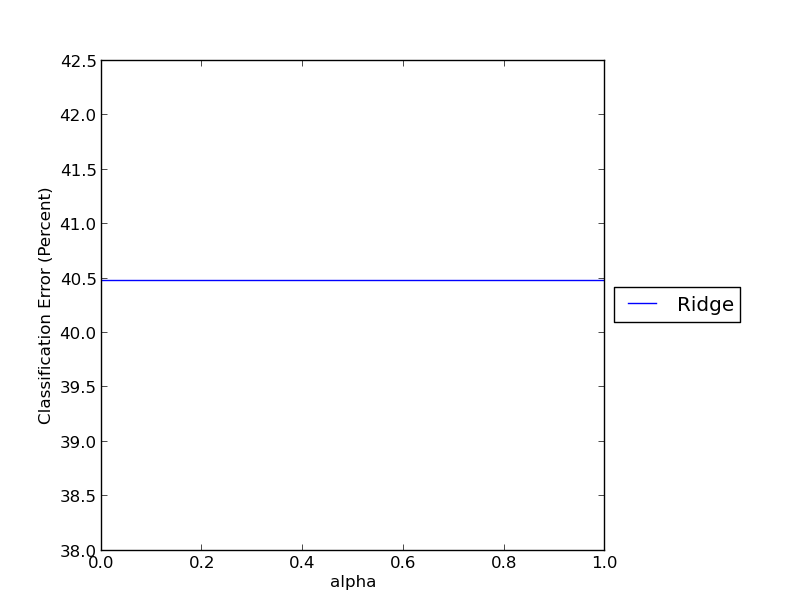
\includegraphics[width=0.8\textwidth]{images/ridgealpha.png}
\caption{The effect on error rate of changing the alpha parameter on Ridge Regression}
\label{fig:ridgealpha}
\end{figure}

\begin{figure}[h!]
\centering
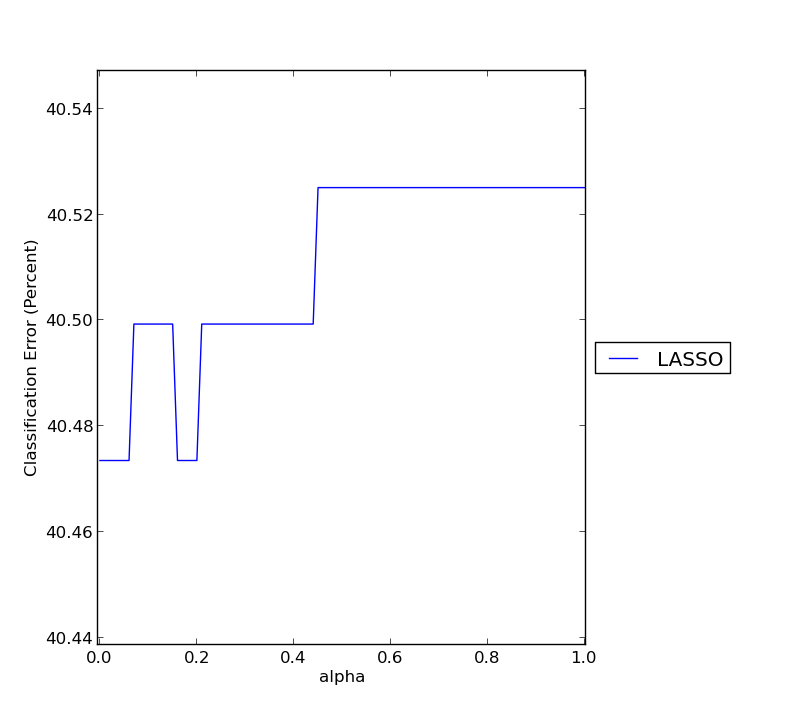
\includegraphics[width=0.8\textwidth]{images/lassoalpha.png}
\caption{The effect on error rate of changing the alpha parameter on LASSO}
\label{fig:lassoalpha}
\end{figure}

\begin{figure}[h!]
\centering
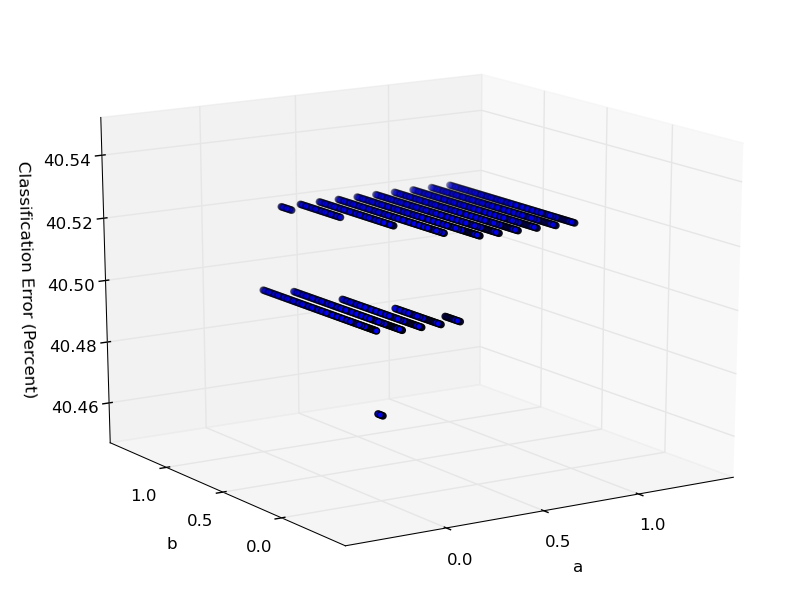
\includegraphics[width=0.8\textwidth]{images/elasticnetab.png}
\caption{The effect on error rate of changing the a and b parameters on Elastic Net}
\label{fig:elasticnetab}
\end{figure}

Figures \ref{fig:ridgealpha}, \ref{fig:lassoalpha} and \ref{fig:elasticnetab} show that none of the parameters have a drastic effect on the error rate of the models. The results for Ridge Regression show no change in the performance of the classifier when changing the parameter, alpha. The following values will be used for these models from now on: Ridge Regression: alpha = 1; LASSO: alpha = 1; ElasticNet: a = 0, b = 0.

\subsubsection{Comparing the Linear Models}
Using the cross-validation method described previously, the 4 different linear models were trained with the parameters discovered via optimisation.

\begin{figure}[h!]
\centering
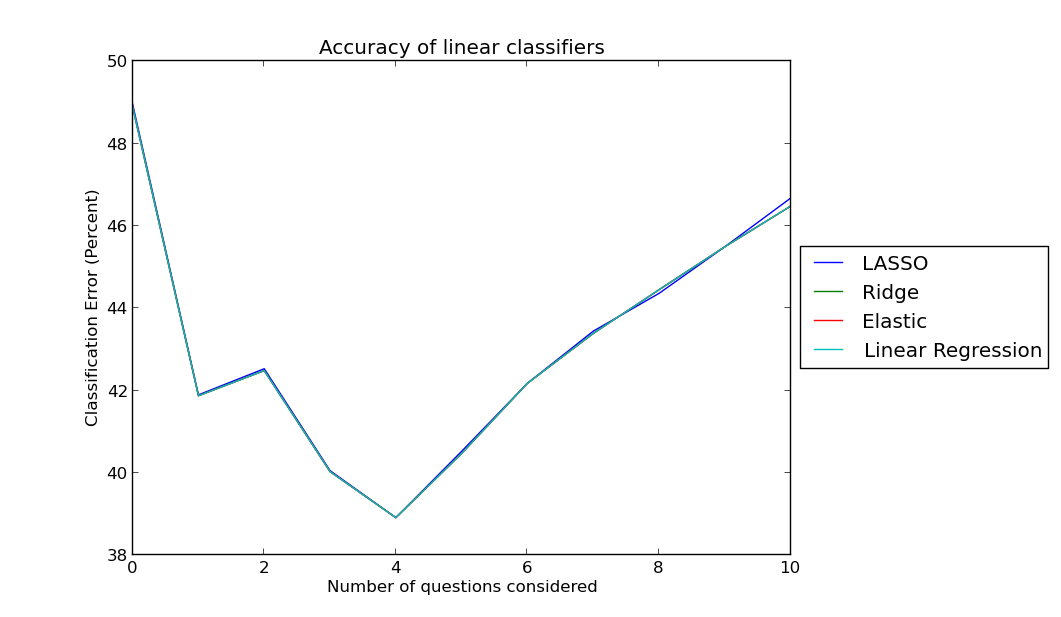
\includegraphics[width=0.8\textwidth]{images/linearmodelsmovingwindow.png}
\caption{The error rates for linear models using the moving window data representation}
\label{fig:linearmodelsmovingwindow}
\end{figure}

\begin{figure}[h!]
\centering
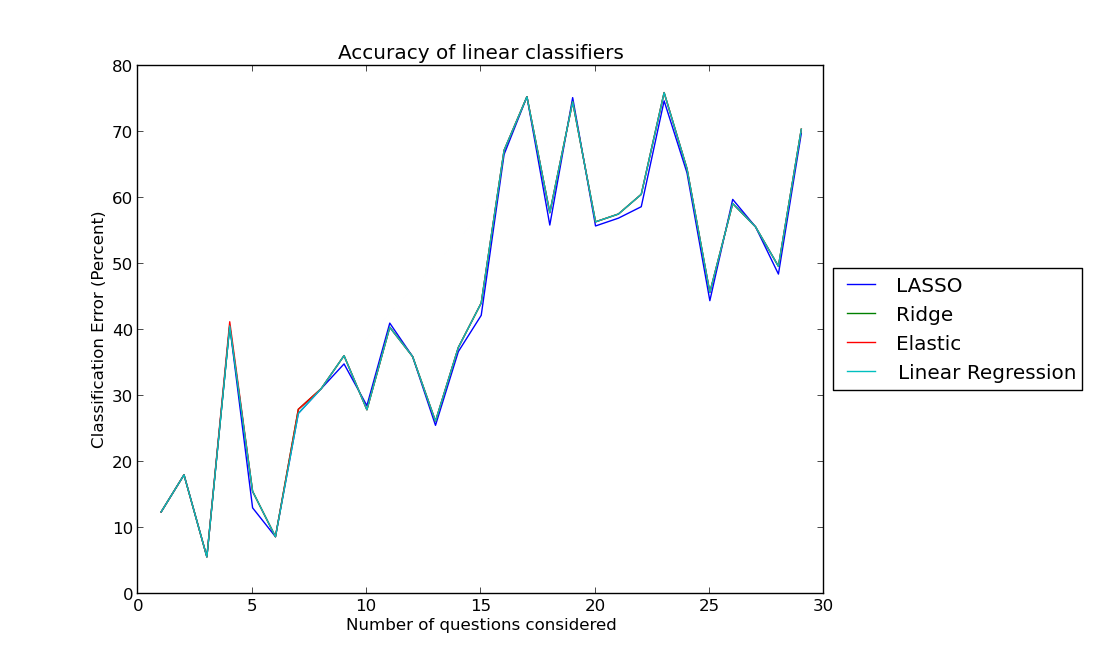
\includegraphics[width=0.8\textwidth]{images/linearmodelsidentified.png}
\caption{The error rates for linear models using the identity based data representation}
\label{fig:linearmodelsidentified}
\end{figure}

Figure \ref{fig:linearmodelsmovingwindow} shows that the performance of the models depends largely on the size of the moving window. For these models the lowest error rate is acheived when the window is of size 4. For this data, the error rate increases as more questions are considered which is at first unexpected: if the model knows more about the previous questions then it should be able to have a more accurate prediction. 

One possible explanation is that the new data is not as relevant. Questions in Infandango are grouped - though not strictly - by the type of the questions: a question is likely to build on knowledge of the previous question. For this reason, results of questions within the same locality are likely to be useful in predicting the results of other questions in the same locality. As this locality is increased the questions become less likely to be relevant to the target question. Not only will these questions add little information, they may also obscure the relevant information from the training algorithms.

Another potential reason for the increasing error rate is that as the window size increases there is less usable data, per observed datapoint, to train on. This is shown in Figure \ref{fig:movingwindowdata}. Less training data means the algorithms have less time to adjust the weights used to predict scores.

\begin{figure}[h!]
\centering
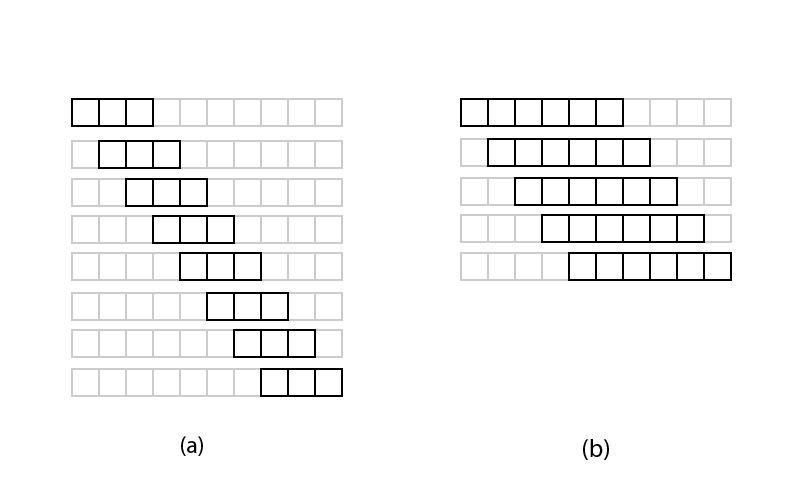
\includegraphics[width=0.8\textwidth]{images/movingwindowdata.png}
\caption{(a) shows how much data can be used with a moving window of size 3 (8 pieces of data), (b) shows the same for a window of size 6 (5 pieces of data).}
\label{fig:movingwindowdata}
\end{figure}

Figure \ref{fig:linearmodelsidentified} shows the lowest error rate when considering 4 questions - interestingly this is the same as the moving window approach. The error rate generally increases as more questions are considered although the behaviour is erratic.
The increase in error rate might be attributed to one of the reasons for the increase in error rate of the moving window approach: as more questions are considered, less of them are relevant.

One factor which might account for both the increase in the error rate and the erratic behaviour is that, in general, this approach will have much less training data than the moving window approach.

As seen in figure \ref{fig:movingwindowdata} the moving window approach can, for one model, train multiple times on the same piece of data. The reason it can do this is that it does not need to consider the identity of the question. However, retaining the identity is exactly how the identity based model differs from the moving window model. For this reason it can only train once on each piece of data, whereas the moving window approach might receive 20 pieces of data from one observed item.

\subsubsection{Conclusion of Linear Models}
One interesting feature of the results so far is that all the linear models behave very similarly on both data representations. Since the graphs do not give any obvious indications of the best model, the averages have been calculated for each model for each data representation, shown in Table \ref{table:linearmodelsaverages}.

The lowest average is shared by Linear Regression, Ridge Regression and Elastic Net. Since Ridge Regression and Elastic Net are Linear Regression with added regularisation, the simpler option will be chosen. Therefore the best Linear model is Linear Regression using the Moving Window approach.

\begin{figure}[h!]
\centering
\begin{tabular}{l || l | l}
Models & Moving Window & Identity based \\ \hline \hline
Linear Regression & 43.1508290455 & 44.066091954 \\ \hline
Ridge Regression & 43.1508290455 & 44.0876436782 \\ \hline
LASSO & 43.1844660458 & 43.5512452107 \\ \hline
Elastic Net & 43.1508290455 & 44.1091954023 \\ \hline
\end{tabular}
\caption{Average error rate for the linear models on two different data representations}
\label{table:linearmodelsaverages}
\end{figure}

\subsection{Support Vector Machines}
A Support Vector Machine is an algorithm that attempts to find a maximum margin hyperplane, which is defined by the {\it support vectors}: the vectors which lie the same distance (margin) away from the hyperplane. This margin is maximised so that the hyperplane lies as far away from each class as possible. A new data point is labelled depending on what side of the hyperplane it lies on. Figure \ref{fig:hyperplane} shows an example hyperplane on two dimensional data, although SVM can work on any number of dimensions.

\begin{figure}[h!]
\centering
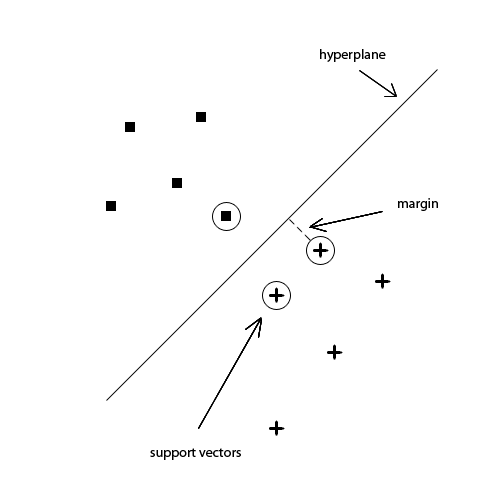
\includegraphics[width=0.8\textwidth]{images/hyperplane.png}
\caption{A maximum margin hyperplane that separates two classes in a two dimensional space}
\label{fig:hyperplane}
\end{figure}

\subsubsection{Kernel Functions}
The simplest, linear Support Vector Machines attempt to find a maximum margin hyperplane using a method which requires calculating the dot product between vectors. In the linear case, the standard dot product is enough to allow the data to be separated. However, if the data is more complex it may not be the approriate function to use. Changing this dot product to be some other function (which must take two vectors and return a scalar value) is what is known as the "kernel trick". The candidate functions are known as kernel functions, and allow for the SVMs to be applied to non-linear data. 

\subsubsection{Optimisation}
Scikit provides 4 preset kernel functions: linear, polynomial, rbf (radial basis function) and sigmoid. In the case of polynomial and sigmoid kernels, an additional parameter, "degree", allows the specification of the degree of the kernel. An appropriate way of finding good values for this parameter is to start at 1, and increase until the estimated error ceases to improve \cite{witten2011data}. 

\begin{figure}[h!]
\centering
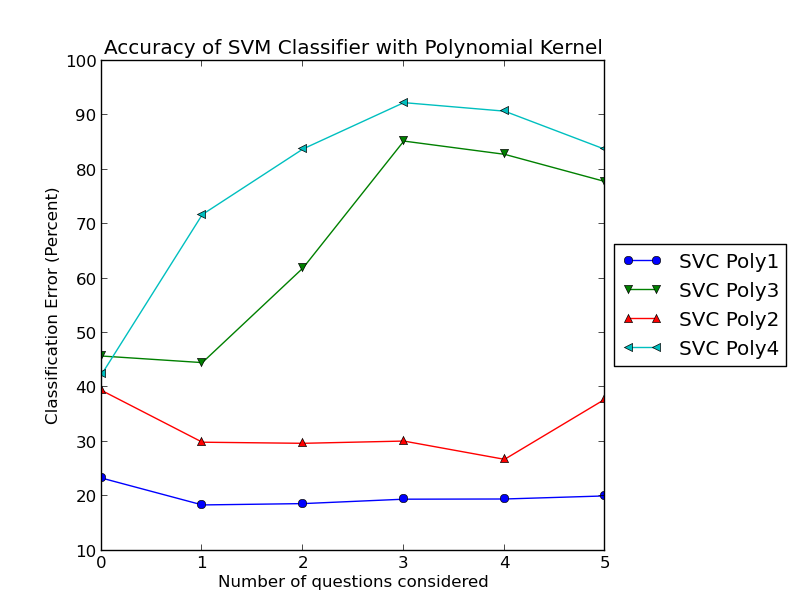
\includegraphics[width=0.8\textwidth]{images/svcpoly.png}
\caption{The performance of a SVM classifier using a polynomial kernel with different degree values}
\label{fig:svcpoly}
\end{figure}

\begin{figure}[h!]
\centering
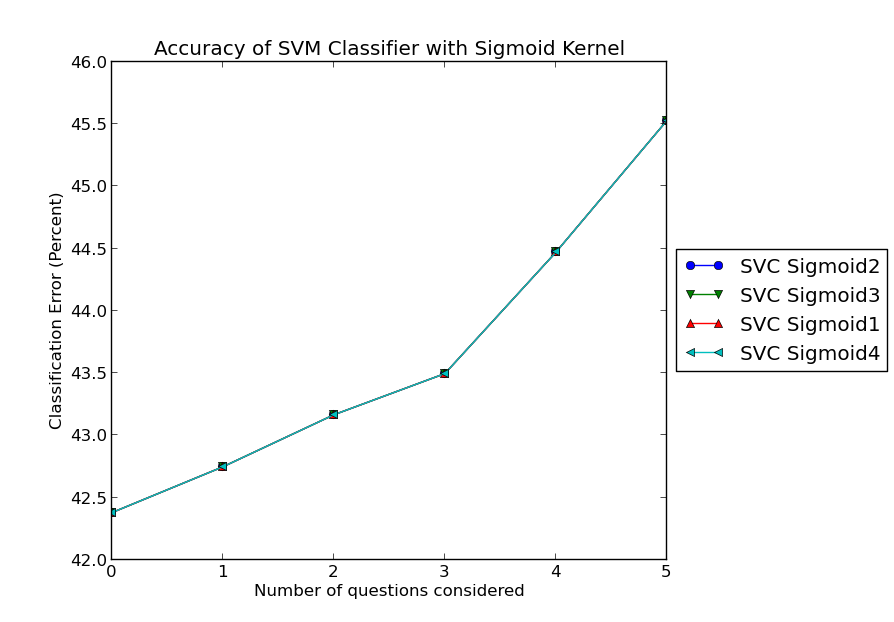
\includegraphics[width=0.8\textwidth]{images/svcsigmoid.png}
\caption{The performance of a SVM classifier using a sigmod kernel with different degree values}
\label{fig:svcsigmoid}
\end{figure}

\begin{figure}[h!]
\centering
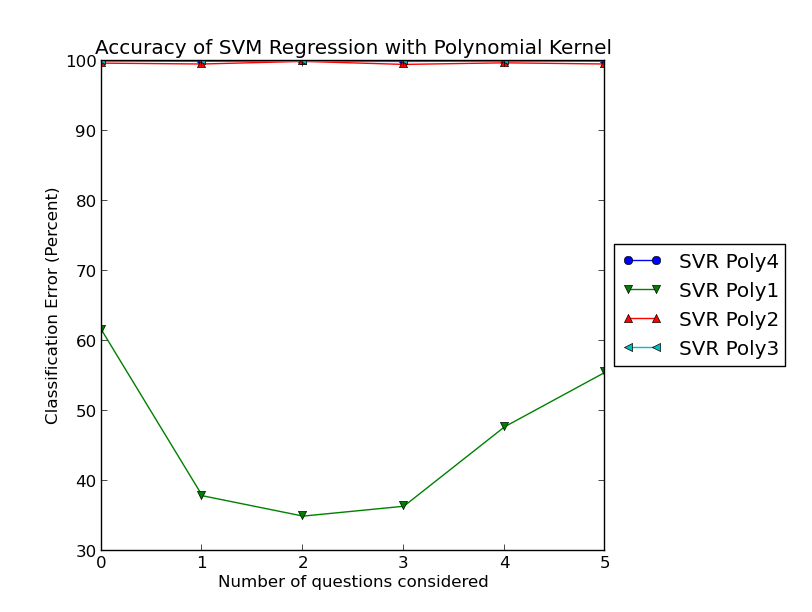
\includegraphics[width=0.8\textwidth]{images/svrpoly.png}
\caption{The performance of a SVM regression using a polynomial kernel with different degree values}
\label{fig:svrpoly}
\end{figure}

\begin{figure}[h!]
\centering
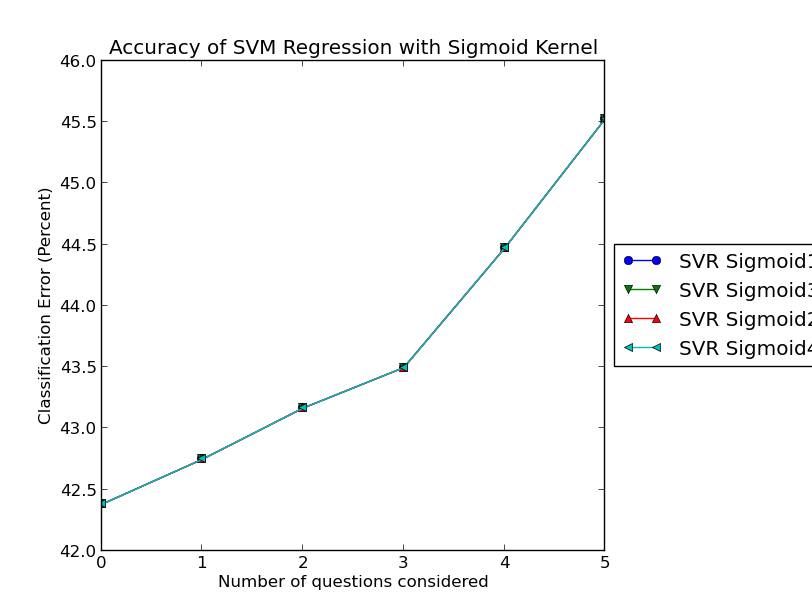
\includegraphics[width=0.8\textwidth]{images/svrsigmoid.png}
\caption{The performance of a SVM regression using a sigmoid kernel with different degree values}
\label{fig:svrsigmoid}
\end{figure}

Figures \ref{fig:svcsigmoid} and \ref{fig:svrsigmoid} show the effect of changing the degree of the sigmoid kernel. In both cases, changing the degree has no effect on the performance of the model. Figures \ref{fig:svcpoly} and \ref{fig:svrpoly} show the effect of changing the degree of a polynomial kernel. Here, changing the degree has a significant affect. In both cases the best value is 1, with the other values performing significantly worse.

\subsubsection{Results}
With the optimisations completed, the different models could be compared against each other. Figure \ref{fig:svmsmovingwindow} and Table \ref{table:svmsmovingwindowaverages} show the results for the moving window approach. Figure \ref{fig:svmsidentified} and Table \ref{table:svmsidentityaverages} show the results for the identity based approach. 
The moving window approach has three similarly high performing models: SVC Linear, SVC Poly, SVC RBF. These models show a very similar performance in the identity based approach, although as with all models their performance is more erratic.

\begin{figure}[h!]
\centering
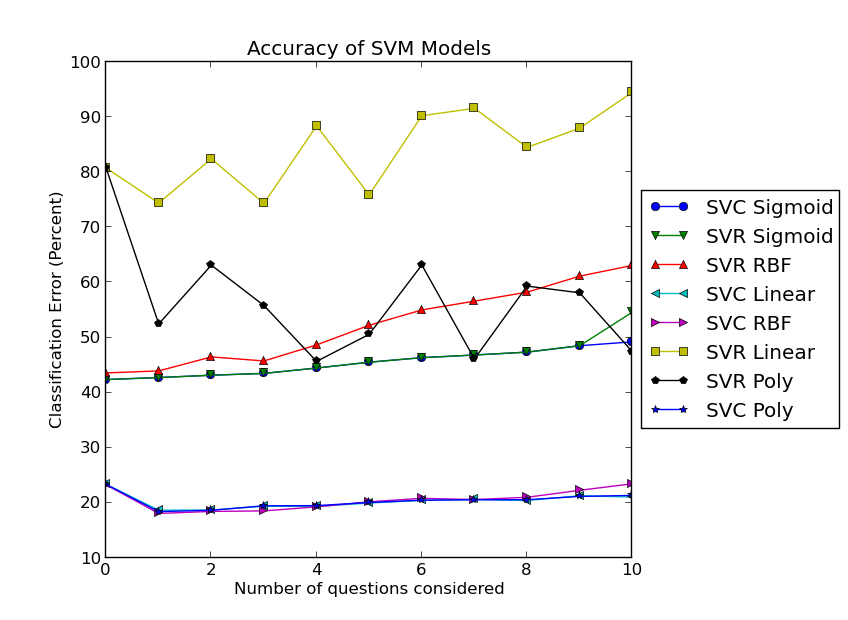
\includegraphics[width=0.8\textwidth]{images/svmsmovingwindow.png}
\caption{The performance of various SVM models}
\label{fig:svmsmovingwindow}
\end{figure}

\begin{figure}[h!]
\centering
\begin{tabular}{l || l }
Models & Average Error \\ \hline \hline
SVC Linear & 20.3041791411 \\ \hline
SVC Poly & 20.3313952482 \\ \hline
SVC RBF & 20.5499438422 \\ \hline
SVC Sigmoid & 45.4603396387 \\ \hline
SVR Sigmoid & 45.9489389873 \\ \hline
SVR RBF & 52.2508272032 \\ \hline
SVR Poly & 56.6047985482 \\ \hline
SVR Linear & 84.1041319495 \\ \hline

\end{tabular}
\caption{Average error rate for SVMs using the moving window approach}
\label{table:svmsmovingwindowaverages}
\end{figure}


\begin{figure}[h!]
\centering
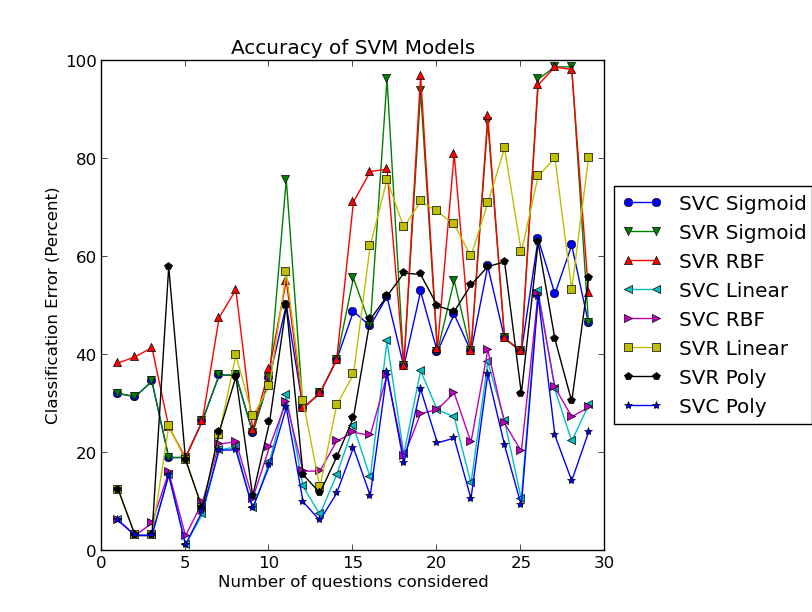
\includegraphics[width=0.8\textwidth]{images/svmsidentified.png}
\caption{The performance of various SVM models}
\label{fig:svmsidentified}
\end{figure}

\begin{figure}[h!]
\centering
\begin{tabular}{l || l }
Models & Average Error \\ \hline \hline
SVC Linear & 20.5459770115 \\ \hline
SVC Poly & 17.8424329502 \\ \hline
SVC RBF & 22.3659003831 \\ \hline
SVR Poly & 35.5555555556 \\ \hline
SVC Sigmoid & 40.6082375479 \\ \hline
SVR Linear & 46.1206896552 \\ \hline
SVR Sigmoid & 49.8970306513 \\ \hline
SVR RBF & 53.43151341 \\ \hline

\end{tabular}
\caption{Average error rate for SVMs using the moving identity based approach}
\label{table:svmsidentityaverages}
\end{figure}

\subsubsection{Conclusion}
3 models perform very similarly on both approaches which makes choosing between them more difficult, although it is at least clear that it should be a classifier. Due to having the lowest combined average, the model chosen as the best SVM is classification with a polynomial kernel of degree 1.

\subsection{Artificial Neural Network}
The ANN implementation used for this project is provided by the Pybrain library. An ANN takes the inputs, passes all the inputs to each unit in a "hidden" layer and the outputs of each unit in the hidden layer are passed to the output units. The units in the hidden layer are artificial neurons and can be of various types. For example, a neuron could be the weighted sum of the inputs. Figure \ref{fig:nn} shows how an ANN suitable for this problem might look. 

\begin{figure}[h!]
\centering
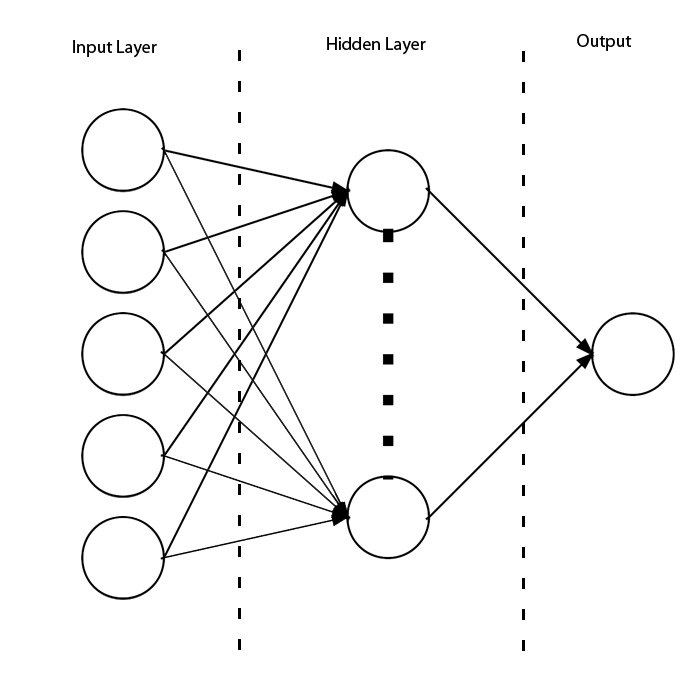
\includegraphics[width=0.8\textwidth]{images/nn.png}
\caption{The topology of an Artificial Neural Network with 5 inputs, one hidden layer with an unspecified number of units and one output unit.}
\label{fig:nn}
\end{figure}

Since Pybrain is a library which focuses specifically on ANNs it has even more customisation than scikit-learn does for its models. The two parameters investigated are the type of units in the hidden layer and the number of units in the hidden. Changing these parameters allows the model to be as complex as the problem requires.

\subsubsection{Optimisation}
Pybrain provides many types of hidden layer, including GaussianLayer, LinearLayer, SigmoidLayer and TanhLayer. Due to technical issues which will be discussed in Chatper \ref{implementation} the layers chosen were SigmoidLayer and TanhLayer.

\subsubsection{Results}
Figure \ref{fig:nnall200} shows how different parameters effect the error of the model. Both models perform similarly except the TanhLayer has a large drop in error rate with 130 hidden units.

\begin{figure}[h!]
\centering
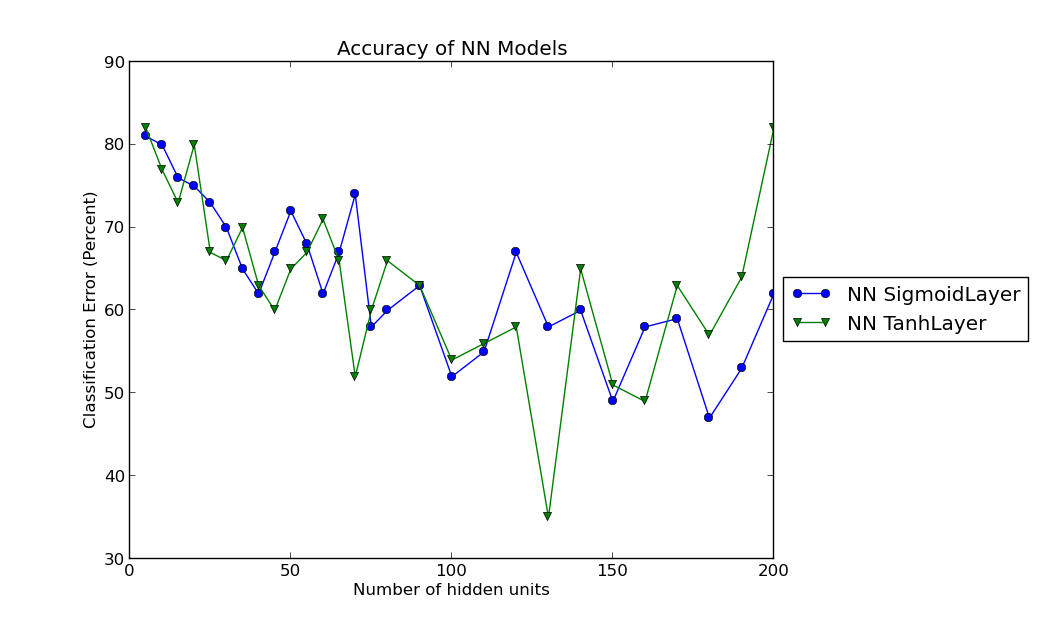
\includegraphics[width=0.8\textwidth]{images/nnall200.png}
\caption{The effect of changing the number of hidden units on Neural Networks with two different hidden layer types.}
\label{fig:nnall200}
\end{figure}

\subsubsection{Conclusion}
There is little to choose between both models, as both have the same general trend and neither performs consistently better than the other. Although it is possibly an anomaly, the model chosen is Artificial Neural Network with Sigmoid squashing function as the hidden layer type with 130 hidden units.

\subsection{Final Model Selection}
The final task is to choose the model that is going to be used in the system. To do this, each of the models are trained and tested on both data representations. Each model uses the parameters determined through optimisation.

\subsubsection{Baseline}
To see if the machine learning actually learns anything that a simple estimate could not have achieved, a baseline is used. The baseline used is simple and intuitive: take the average of the available features. By measuring the accuracy of the models against this baseline we can see if performing machine learning is worthwhile.

\subsubsection{Results}
The models from the previous sections are trained and tested alongside the baseline for both data representations.

\begin{figure}[h!]
\centering
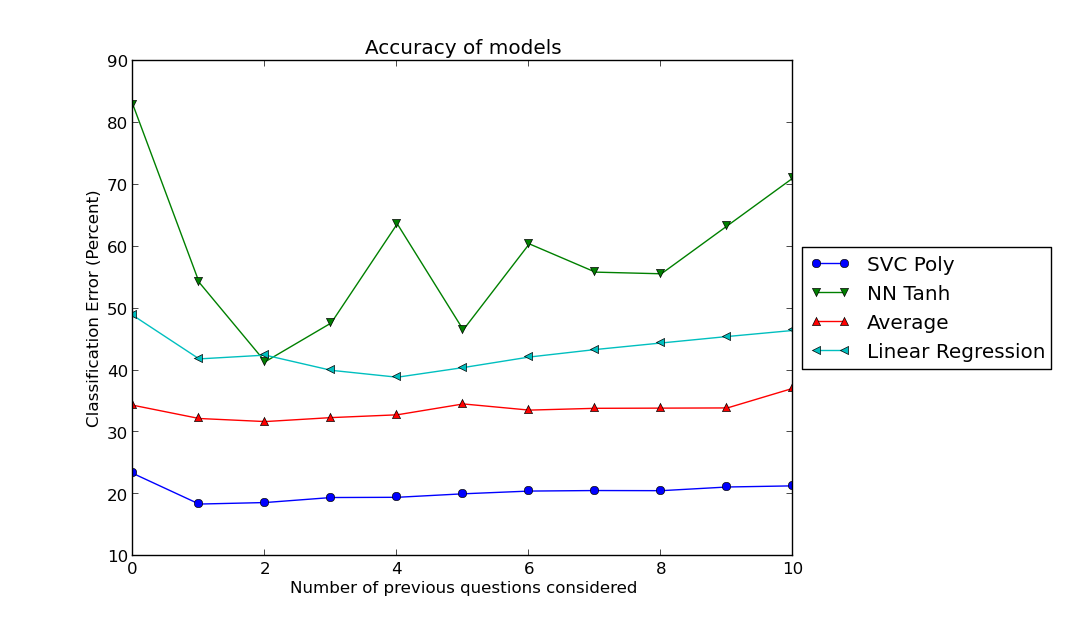
\includegraphics[width=0.8\textwidth]{images/finalmovingwindow.png}
\caption{The performance of the optimised models using the moving window approach}
\label{fig:finalmovingwindow}
\end{figure}

\begin{figure}[h!]
\centering
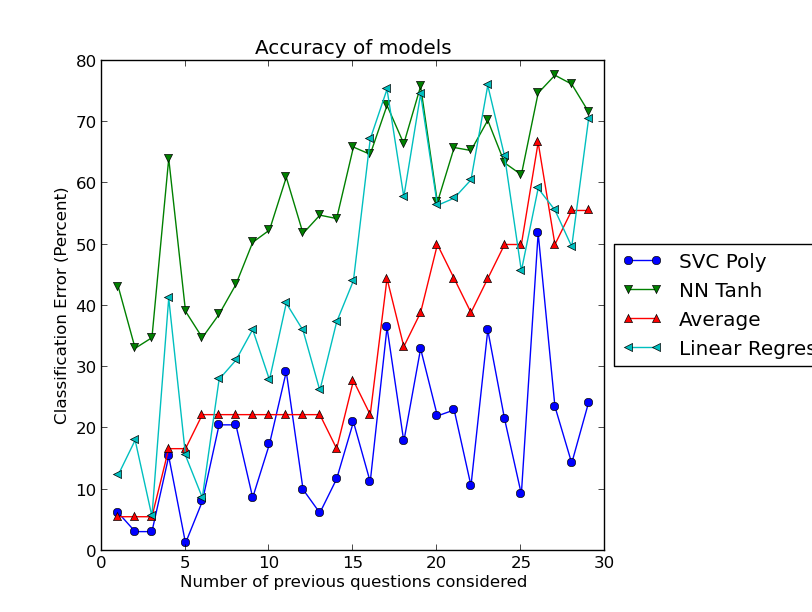
\includegraphics[width=0.8\textwidth]{images/finalidentified.png}
\caption{The performance of the optimised models using the identity based approach}
\label{fig:finalidentified}
\end{figure}

Figure \ref{fig:finalmovingwindow} shows the error of the models on the moving window approach. A clear ordering can be seen in which only the support vector machine performs better than the baseline. 

Figure \ref{fig:finalidentified} shows the error of the models on the identity based approach. All classifiers show a much less consistent performance on this data representation though the general trend remains the same as in the previous approach. 

\subsubsection{Conclusion}
Through a process of optimisations the best models were chosen for each machine learning algorithm. These models then had their performance measured against a baseline, which proved that only the support vector machien performed better than simply taking the average of the available submissions. The moving window approach maintains a consistent performance across all the questions. The identity based approach shows erratic behaviour which sometimes performs better than the moving window approach but sometimes performs worse. On average the models perform quite similarly and due to the implementation advantages of the moving window approach (Chapter \ref{design}) the final model is a Support Vector Classifier using a polynomial kernel of degree 1 on the moving window approach.
